\newcommand{\DiagramScale}{0.6}
\chapter{PCL Compiler}
PLCc is the PCL compiler. It is located in the \texttt{src/pclc} directory of the Git clone and your path should be set according. This chapter introduces the PCL syntax using \emph{railroad diagrams}. Railroad diagrams illustrate valid PCL and are read from left to right, following the lines as a train would. The symbols in the yellow ovals are to be typed \emph{as is}. The symbols in the tan rectangles references another railroad diagram. The referenced diagram should be used to expand the rectangle in more valid PCL. Hexagons contain \emph{character classes} and specify a range of characters that will be accepted.

\section{PCL Syntax}
PCL is a free-form language which allows the programmer to use arbitrary white-space to format your component definitions. Comments are a single line and should start with the \texttt{\#} and can appear at any point in a PCL file.
\begin{figure}[h!]
  \centering
    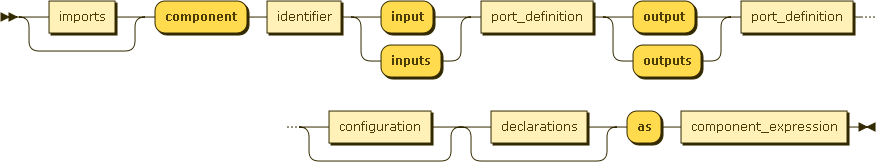
\includegraphics[scale=\DiagramScale,angle=90]{chapters/compiler/diagrams/component}
  \caption{PCL file syntax.}
  \label{fig:pcl-top-level}
\end{figure}
The top level syntax of a PCL file is shown in Figure \ref{fig:pcl-top-level}, and consists of the following sections:
\begin{itemize}
\item \textbf{Imports}: Imports can be optionally specified. Importing, as in other language, makes available other components to the PCL component being written.
\item \textbf{Component}: This starts the component definition and provides the name. The component's name must be the same as the filename. E.g., a component in \texttt{fred.pcl} must be called \texttt{fred}.
\item \textbf{Inputs}: Defines the inputs of the component. This information is used to verify that the outputs of a previous component is compatible with another.
\item \textbf{Outputs}: Defines the outputs of the component. This information is used to verify that the inputs of a subsequent component is compatible with another.
\item \textbf{Configuration}: Optional configuration for the component. This is static data that shall be used to construct imported components used in this component. 
\item \textbf{Declarations}: Optional declarations of components used in this component. This is where the import components are constructed.
\item \textbf{Definition}: This portion is the component definition. It is an expression which defines how the constructed components are to be combined to create the computation required.
\end{itemize}

\subsection{Imports}\label{subsec:imports}
\begin{figure}[h!]
  \centering
    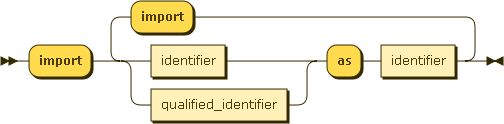
\includegraphics[scale=\DiagramScale]{chapters/compiler/diagrams/imports}
  \caption{\texttt{imports} : Importing PCL files.}
  \label{fig:pcl-imports}
\end{figure}
Extant PCL components can be used in other PCL components. The mechanism for using components is through importing. There can be zero or more imports in a PCL file. Figure \ref{fig:pcl-imports} shows the syntax for importing.

The imported component is referenced using an identifier which can be fully qualified using a dot separated name. If the component is referenced using one or more dots the sequence of identifiers, apart from the last one, is used to address a package of components. The last identifier specifies the component name. The environment variable \texttt{PCL\_IMPORT\_PATH} is a colon separated list of directories from which a search shall take place for the PCL components. If this environment variable is not set then the current working directory is used as a starting point for the component search.

Each imported component must specify an alias. This is the name by which this component shall be referred to in this PCL file. E.g., \texttt{import components.utility.sleep as sleep\_comp} shall import a PCL component called \texttt{sleep} from the package \texttt{components.utility} and shall be refereed to as, i.e. has the alias, \texttt{sleep\_comp}.

\subsection{Port Definition}\label{subsec:port-def}
\begin{figure}[h!]
  \centering
    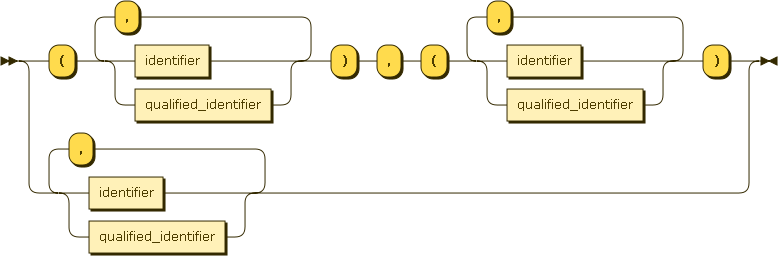
\includegraphics[scale=\DiagramScale,angle=90]{chapters/compiler/diagrams/port_definition}
  \caption{\texttt{port\_definition} : Component port definition.}
  \label{fig:pcl-port-def}
\end{figure}
A port definition informs the PCL compiler about the nature of a component's input or an output. Components can have 2, 3 or 4 ports: one input and output port, one input port and two output ports, two input ports and one output port, or two input and output ports. Figure \ref{fig:pcl-port-def} shows the syntax for this grammatical construct.

A port can carry one or more \emph{signals}. A signal is a piece of data that flows through ports and has a unique name to that port, and can be fully qualified\footnote{It may be easier to group signals through the use of a hierarchical naming convention, e.g., \texttt{a.b.c} and \texttt{a.b.d}.}. The signal names, for a port, are declared in a port definition. The ``shape'' of a port definition declares whether an input or an output has one or two ports. For example, consider the following input and output port definitions:
\begin{itemize}
\item A component with one input and one output port. Input signals are \texttt{tom}, \texttt{dick}, \texttt{harry} and output signals are \texttt{disley} and \texttt{standedge}.
\begin{center}
\begin{verbatim}
component tunnel
    inputs tom, dick, harry
    outputs disley, standedge
    ...
\end{verbatim}
\end{center}

\item A component with one input and two output ports. Input signal is \texttt{fruit.banana}. The \emph{top} output port signal is \texttt{veg.carrot} and the \emph{bottom} output port signals are \texttt{fruit.super}, and \texttt{fruit.salad}.
\begin{center}
\begin{verbatim}
component split
    inputs fruit.banana
    outputs ( veg.carrot ), ( fruit.super, fruit.salad )
    ...
\end{verbatim}
\end{center}

\item A component with two inputs and one output port. Input signals for the \emph{top} port are \texttt{tea} and \texttt{coffee}, and the signals for the \emph{bottom} port are \texttt{milk}, and \texttt{water}. The output port's single signal is \texttt{drink}.
\begin{center}
\begin{verbatim}
component pot
    inputs ( tea, coffee ), ( milk, water )
    outputs drink
    ...
\end{verbatim}
\end{center}

\item A component with two input and output ports. Input signals for the \emph{top} port are \texttt{zippy} and \texttt{george}, and the signals for the \emph{bottom} port are \texttt{rod}, \texttt{jane}, and \texttt{freddy}. The output signals are for the \emph{top} port are \texttt{geoffrey}, and the \emph{bottom} port signals are \texttt{bungle} and \texttt{zippo}.
\begin{center}
\begin{verbatim}
component rainbow
    inputs ( zippy, george ), ( rod, jane, freddy )
    outputs ( geoffrey ), ( bungle, zippo )
    ...
\end{verbatim}
\end{center}

\end {itemize}

\subsection{Configuration}\label{subsec:config}
\begin{figure}[h!]
  \centering
    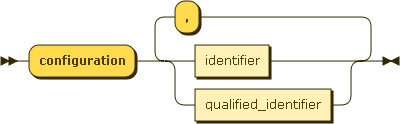
\includegraphics[scale=\DiagramScale]{chapters/compiler/diagrams/configuration}
  \caption{\texttt{configuration} : Component configuration.}
  \label{fig:pcl-config}
\end{figure}
A component's configuration is static data that is primarily used for constructing import components. Configuration data is named using identifiers, which can be fully qualified. Figure \ref{fig:pcl-config} shows the configuration syntax. Configuration identifiers may also be used in \emph{if} components see Section \ref{sec:if} for details. A PCL can declare zero or more configuration identifiers.

Figure \ref{fig:pcl-config-example} shows an example of configuration being declared in a PCL file. Here the \texttt{parallel\_sleep} component shall be constructed using two configuration values, namely \texttt{sleep\_command} and \texttt{sleep\_time}.
\begin{figure}[h!]
\begin{center}
\begin{verbatim}
import sleep as sleep

component parallel_sleep
    ...
    configuration sleep_command, sleep_time
    ...
\end{verbatim}
\end{center}
\caption{Example declaration of PCL configuration.}
\label{fig:pcl-config-example}
\end{figure}

\subsection{Declarations}\label{subsec:decls}
\begin{figure}[h!]
  \centering
    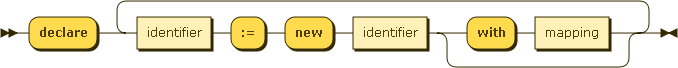
\includegraphics[scale=0.45]{chapters/compiler/diagrams/declarations}
  \caption{\texttt{declarations} : Imported component construction.}
  \label{fig:pcl-decls}
\end{figure}
The declaration section of a PCL file is where the imported components can be constructed using the configuration available in the importing component's PCL. Figure \ref{fig:pcl-decls} shows the syntax for component construction. All declarations are assigned to an identifier which shall be unique. The import alias (see Section \ref{subsec:imports}) is used to reference the imported component from which an instance is created. There is an optional \emph{with} clause which allows configuration to be mapped into a component's constructor. Figure \ref{fig:pcl-config-mapping} shows the configuration mapping syntax
\begin{figure}[h!]
  \centering
    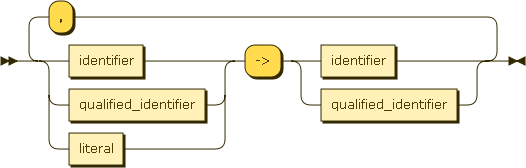
\includegraphics[scale=\DiagramScale]{chapters/compiler/diagrams/configuration_mapping}
  \caption{\texttt{configuration\_mapping} : Declaration configuration mapping}
  \label{fig:pcl-config-mapping}
\end{figure}


The PCL snippet in Figure \ref{fig:pcl-decl-example} shows an example of constructing imported components.
\begin{figure}[h!]
\begin{center}
\begin{verbatim}
import sleep as sleep_component
import message as message_component

component parallel_sleep
    input sleep_time
    outputs (complete), (complete)
    configuration sleep_command
    declare
        top_sleep := new sleep_component
            with sleep_command -> command.sleep
        bottom_sleep := new sleep_component
            with sleep_command -> command.sleep
        message_world := new message_component
    ...
\end{verbatim}
\end{center}
\caption{Example of component construction.}
\label{fig:pcl-decl-example}
\end{figure}
Here two instances of the same component are constructed, namely the \texttt{sleep} component, which has the alias \texttt{sleep\_component}. The \texttt{sleep} component specifies the configuration \texttt{command.sleep} so the \emph{with} clause maps the \texttt{parallel\_sleep} component's configuration to the \texttt{sleep} component's configuration. The \texttt{message} component, on the other hand, requires no configuration in order to construct it.

\subsection{Definition}
This section of the PCL file is where the component's computation is to be defined. The components constructed in the declarations are to be combined to produce a composite component. Figure \ref{fig:pcl-def} shows the recursive syntax, which builds a single expression, for this section.
\begin{figure}[h!]
  \centering
    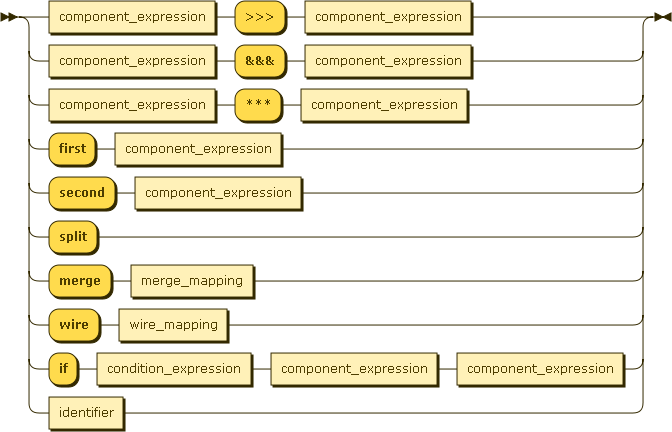
\includegraphics[scale=\DiagramScale,angle=90]{chapters/compiler/diagrams/component_expression}
  \caption{\texttt{component\_expression} : Component definition.}
  \label{fig:pcl-def}
\end{figure}

\subsubsection{Composition}
The \texttt{>>>} combinator sequences two components, one after the other. For example \texttt{comp\_one >>> comp\_two} will produce a component which will apply the output of \texttt{comp\_one} to the input of \texttt{comp\_two}.

Consider two components both with one input and output port, the first component, $c_1$, has an input signal called \texttt{b} and output signal called \texttt{c}, and the second component, $c_2$, has an input signal called \texttt{c} and an output signal called \texttt{d}. Then composing these components, $c_1 >>> c_2$, yields a component whose input signal is called \texttt{b} and an output signal called \texttt{d}.

In order for the components to compose the output of the left-hand side must be compatible with the input of the right-hand side. That is, the number of ports must be identical and the signals must correspond. PCLc will produce an error during compilation if the components are not compatible.

\subsubsection{First}
The \texttt{first} combinator takes a single component and produces a two input and output port component. The \emph{top}, or \emph{first}, element of the input is applied to the component, whilst the \emph{bottom}, or \emph{second}, input element passes through the resultant component untouched. This second input signal's value is remembered across the computation of the provided component.

Consider a component, $c$, with one input and one output port whose signals are \texttt{b} and \texttt{c} respectively. Applying the \texttt{first} combinator to $c$, with $first\ c$, yields a component that has two input ports with the port specification $(b), (d)$, and two output ports with specification, $(c), (d)$.

\subsubsection{Second}
The \texttt{second} combinator takes a single component and produces a two input and output port component. The \emph{bottom}, or \emph{second}, element of the input is applied to the component, whilst the \emph{top}, or \emph{first}, input element passes through the resultant component untouched. This first input signal's value is remembered across the computation of the provided component.

Consider a component, $c$, with one input and one output port whose signals are \texttt{b} and \texttt{c} respectively. Applying the \texttt{second} combinator to $c$, with $second\ c$, yields a component that has two input ports with the port specification $(d), (b)$, and two output ports with specification, $(d), (c)$.

\subsubsection{Parallel}
The \texttt{***} combinator composes two components such that they run in \emph{parallel}. This combinator is best explained in terms of the first, second and composition combinators. Thus,
\begin{center}
$a\ ***\ b\ =\ first\ a\ >>>\ second\ b$
\end{center}
Hence, for two components:
\begin{itemize}
\item $c_1$: One input port, with port specification $b$, and one output port, with specification $c$, and
\item $c_2$: One input port, with port specification $d$, and one output port, with specification $e$.
\end{itemize}
Then $c_1\ ***\ c_2$ shall yield a two input and output port component with:
\begin{itemize}
\item Input port specification $(b), (d)$, and
\item Output port specification $(c), (e)$.
\end{itemize}

\subsubsection{Split}
Split is a pre-defined component which has one input port and two output ports. Split simply takes the signals on it's input and copies them to both output ports. Hence, \emph{splitting} the input to the output.

\subsubsection{Fanout}
The \texttt{\&\&\&} combinator yields a component with one input port and two output ports. It is defined as:
\begin{center}
$a\ \&\&\&\ b\ =\ split\ >>>\ (first\ a\ ***\ second\ b)$
\end{center}
Since \texttt{split} is begin used both components, $a$ and $b$, require their input port signals to be compatible with the input to split.

Consider two components:
\begin{itemize}
\item $c_1$: One input port, with port specification $b$, and one output port, with specification $c$, and
\item $c_2$: One input port, with port specification $b$, and one output port, with specification $d$.
\end{itemize}
Then $c_1\ \&\&\&\ c_2$ shall yield a one input and two output port component with:
\begin{itemize}
\item Input port specification $b$, and
\item Output port specification $(c), (d)$.
\end{itemize}

PCLc verifies that components, used with the fanout combinator, have compatible ports and signals. The compiler will report errors if there are incompatible components used.

\subsubsection{Merge}\label{subsubsec:merge}
The merge component is a pre-defined component that expects a mapping and \emph{merges} the output from a two output port component to a single port component. Hence, a merge component has two input ports and one output port.

The merge mapping syntax is shown in Figure \ref{fig:pcl-merge-mapping}.
\begin{figure}[h!]
  \centering
    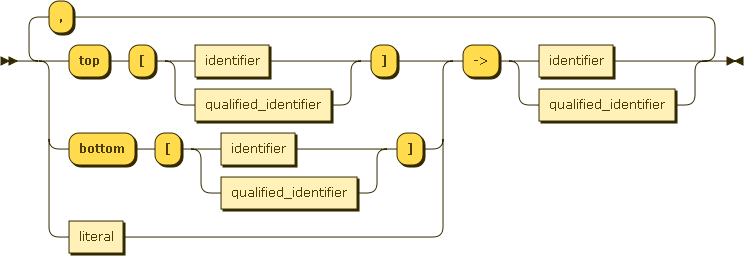
\includegraphics[scale=\DiagramScale,angle=90]{chapters/compiler/diagrams/merge_mapping}
  \caption{\texttt{merge\_mapping} : Merge component mapping.}
  \label{fig:pcl-merge-mapping}
\end{figure}
The merge mapping specifies which signals from the \emph{top} and \emph{bottom} input ports shall be mapped to the output port to uniquely named signals. Constant values can also be introduced to the output. Further to this, signals can be dropped, that is, a signal that is not passed onto the subsequent component.

Consider a component with two output ports, with the following port specification
\begin{center}
$(src.file.name,\ src.file.size),\ (obj.file.name,\ obj.file.size)$
\end{center}
that needs merging into a single port, with specification:
\begin{center}
$source\_filename,\ object\_filename,\ source\_language$
\end{center}
The following merge expression could be used:
\begin{center}
  \begin{verbatim}
merge top[src.file.name] -> source_filename,
      top[src.file.size] -> _,
      bottom[obj.file.name] -> object_filename,
      bottom[obj.file.size] -> _,
      "PCL" -> source_language
  \end{verbatim}
\end{center}
This merge mapping does the following:
\begin{itemize}
\item The signal \texttt{src.file.name}, in the \emph{top} input port, is mapped to the output port signal \texttt{source\_filename},
\item The signal \texttt{src.file.size}, in the \emph{top} input port, is dropped and is not present in the output port signals,
\item The signal \texttt{obj.file.name}, in the \emph{bottom} input port, is mapped to the output port signal \texttt{object\_filename},
\item The signal \texttt{obj.file.size}, in the \emph{bottom} input port, is dropped and is not present in the output port signals, and
\item The string literal \texttt{PCL} is mapped into the output port's \texttt{source\_language} signal.
\end{itemize}
Other constant literals can be used in a merge mapping and are described in Section \ref{sec:literals}.

\subsubsection{Wire}\label{subsubsec:wire}
Wire components are used to adapt one component's output signals to match the expected input signals of a subsequent component. Wires can only be used to adapt adjacent components that have an equal number of ports, i.e., the resultant wire component always has the same number of input ports as output ports. The \emph{wire mapping} determines whether a one or two port component is being adapted, this is shown in Figure \ref{fig:pcl-wire-mapping}.
\begin{figure}[h!]
  \centering
    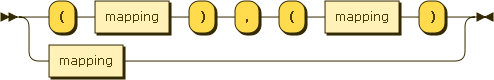
\includegraphics[scale=\DiagramScale]{chapters/compiler/diagrams/wire_mapping}
  \caption{\texttt{wire\_mapping} : Wire mapping.}
  \label{fig:pcl-wire-mapping}
\end{figure}
The mapping syntax is shown in Figure \ref{fig:pcl-mapping}.
\begin{figure}[h!]
  \centering
    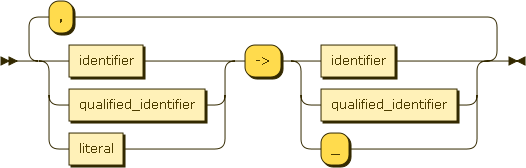
\includegraphics[scale=\DiagramScale]{chapters/compiler/diagrams/mapping}
  \caption{\texttt{mapping} : Mapping.}
  \label{fig:pcl-mapping}
\end{figure}
In common with the merge mapping, signals can be mapped into other signals, dropped, or assigned literal values.

Consider the following wire component:
\begin{center}
  \begin{verbatim}
wire src.file.name -> source_filename,
     src.file.size -> _,
     "PCL" -> source_language
  \end{verbatim}
\end{center}
This mapping adapts two components with one output and one input port with the following port specifications,
\begin{center}
$src.file.name,\ src.file.size$
\end{center}
and
\begin{center}
$source\_filename,\ source\_language$
\end{center}
respectively.

A two input and output port wire is defined thus,
\begin{center}
  \begin{verbatim}
wire (src.file.name -> source_filename,
      src.file.size -> _,
      "PCL" -> source_language),
     (obj.file.name -> object_filename,
      obj.file.size -> _,
      "Python" -> object_language)
  \end{verbatim}
\end{center}
This mapping adapts two components with two output and two input ports with the following port specifications,
\begin{center}
$(src.file.name,\ src.file.size),\ (obj.file.name,\ obj.file.size)$
\end{center}
and
\begin{center}
$(source\_filename,\ source\_language),\ (object\_filename,\ object\_language)$
\end{center}
respectively.

\subsubsection{If}\label{sec:if}
The \emph{if} component provides a mechanism to conditionally execute components in a pipeline. The first argument to the \emph{if} component is a condition expression, the second is the \emph{then} component, and the third is the \emph{else} component. The \emph{then} and \emph{else} components \emph{must}:
\begin{itemize}
\item only specify one input port,
\item specify identical signals on the input ports,
\item have identical numbers of output ports (one or two), and
\item specify identical signals in their output ports.
\end{itemize}

If the condition expression is evaluated to a truthy value the \emph{then} component shall be executed, otherwise the \emph{else} component is executed.
\begin{figure}[h!]
  \centering
    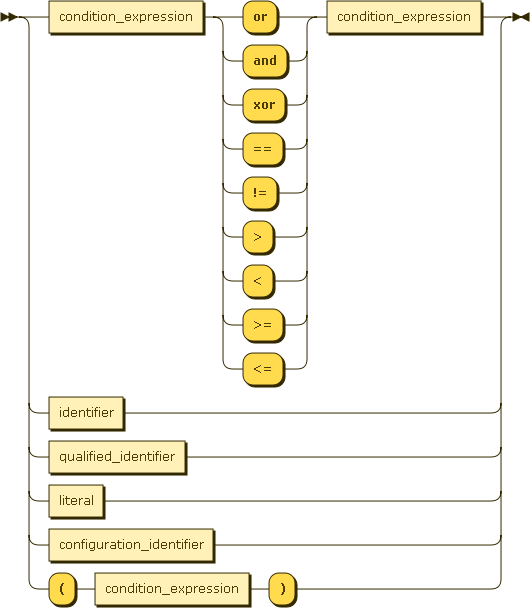
\includegraphics[scale=\DiagramScale]{chapters/compiler/diagrams/condition_expression}
  \caption{\texttt{condition\_expression} : If component's condition expression.}
  \label{fig:pcl-cond-expr}
\end{figure}
In Figure \ref{fig:pcl-cond-expr} the recursive syntax for the condition expression is shown. A condition expression is built up using the logical operators (\texttt{or}, \texttt{and}, and \texttt{xor})\footnote{Hopefully these operators require no explanation.}, and the relational operators (\texttt{==}, \texttt{!=}, \texttt{>}, \texttt{<}, \texttt{>=}, \texttt{<=})\footnote{And these! ;)}. The \texttt{identifier} and \texttt{qualified\_identifier} refer to the signals in the input ports of the \emph{then} and \emph{else} components. Also, configuration identifiers may be used in a condition expression, the grammar of which is shown in Figure \ref{fig:pcl-config-id}.
\begin{figure}[h!]
  \centering
    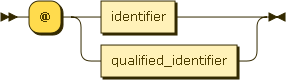
\includegraphics[scale=\DiagramScale]{chapters/compiler/diagrams/configuration_identifier}
  \caption{\texttt{configuration\_identifier} : If component's condition expression configuration identifier.}
  \label{fig:pcl-config-id}
\end{figure}
This allows both the values of input port signals and configuration to be used to decide on which component to execute.

Consider the following PCL snippet:
\begin{center}
  \begin{verbatim}
...
component conditional
  inputs a, b
  outputs z
  configuration f
  ...
  as
    if (a == True or a != b) and @f == False
       then_component
       else_component
    ...
  \end{verbatim}
\end{center}
The \texttt{then\_component} shall only be executed if the input \texttt{a} is true or \texttt{a} and \texttt{b} are equal, and the configuration \texttt{f} is false.

\subsection{Identifier}
In common with other programming languages PCL offers identifiers which can start with a letter or an underscore and then any number of letters, numbers or underscores, or diagrammatically see Figure \ref{fig:pcl-id}.
\begin{figure}[h!]
  \centering
    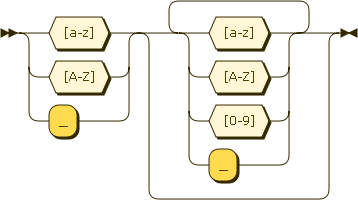
\includegraphics[scale=\DiagramScale]{chapters/compiler/diagrams/identifier}
  \caption{\texttt{identifier} : Identifier.}
  \label{fig:pcl-id}
\end{figure}

\subsection{Qualified Identifier}
Qualified identifiers allows PCL developers to namespace their identifiers using dot separated identifiers, e.g., \texttt{tokeniser.source.filename}. Their syntax is shown in Figure \ref{fig:pcl-qualified-id}.
\begin{figure}[h!]
  \centering
    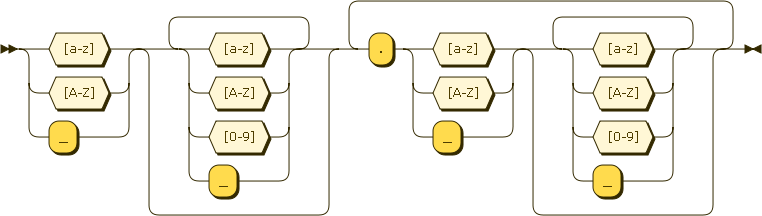
\includegraphics[scale=\DiagramScale,angle=90]{chapters/compiler/diagrams/qualified_identifier}
  \caption{\texttt{qualified\_identifier} : Qualified identifier.}
  \label{fig:pcl-qualified-id}
\end{figure}
Qualified identifiers are available for use in:
\begin{itemize}
\item Imports: qualified identifiers are used to address compiled PCL components (see Section \ref{subsec:imports}),
\item Port definitions: input and output signals can be namespaced for clarity (see Section \ref{subsec:port-def}),
\item Configuration: configuration identifiers can be namespaced for clarity (see Section \ref{subsec:config}),
\item Declarations: configuration mapping may required namespaced configuration to be used (see Section \ref{subsec:decls}),
\item Merge and wire mappings: mapped port can contain namespaced signal names (see Section \ref{subsubsec:merge} and Section \ref{subsubsec:wire} respectively), and
\item \emph{If} conditions: configuration used in \emph{if} condition expressions may be namespaced (see Section \ref{sec:if}).
\end{itemize}

\subsection{Literal}\label{sec:literals}
Literal constants can be used to inject values into component constructors, merge and wire mappings, and \emph{if} condition expressions. They take the form of:
\begin{itemize}
\item Numbers: integer and floating point, e.g., \texttt{-7}, \texttt{2.71828}, \texttt{6.674e-11},
\item Strings: string must be quoted using double quotes (\texttt{"}) and special characters can be escaped using a backslash (\textbackslash), e.g. \texttt{"This is a line of text\textbackslash n"}, and \texttt{"Quoting is \textbackslash"allowed\textbackslash" by escaping the quotes"}, and
\item Booleans: \texttt{true} and \texttt{false}.
\end{itemize}
Figure \ref{fig:pcl-literal} shows their syntax.
\begin{figure}[h!]
  \centering
    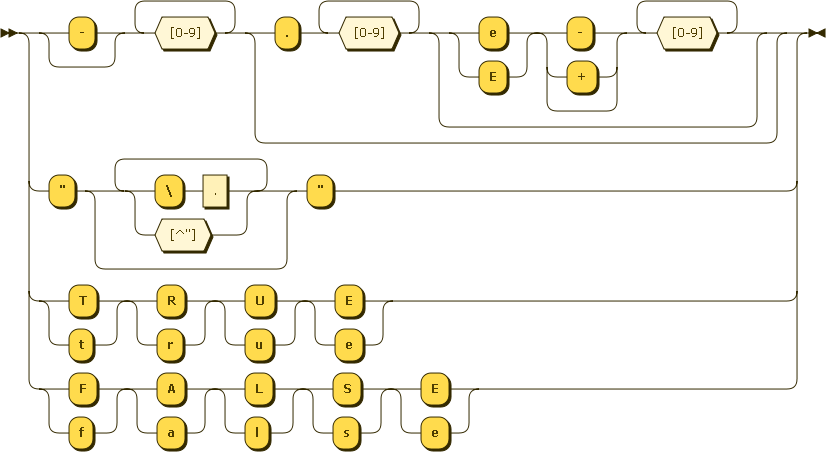
\includegraphics[scale=\DiagramScale,angle=90]{chapters/compiler/diagrams/literal}
  \caption{\texttt{literal} : Literal.}
  \label{fig:pcl-literal}
\end{figure}

\subsection{Example PCL file}
This example PCL file can be found in the \texttt{parallel\_sleep} example PCL.
\begin{figure}[h!]
  \begin{verbatim}
import sleep as sleep

component parallel_sleep
  input sleep_time
  outputs (complete), (complete)
  configuration sleep_command
  declare
    top_sleep := new sleep with sleep_command -> sleep_command
    bottom_sleep := new sleep with sleep_command -> sleep_command
  as
    top_sleep &&& bottom_sleep
  \end{verbatim}
  \caption{Example PCL file.}
\end{figure}
This component constructs two sleep components using a static sleep command to execute. The two sleep components are composed using the fanout operation, such that they run in parallel. Other example PCL files can be found in the \texttt{examples} directory of your Git clone.

\section{Usage}\label{sec:pclc-usage}
Ensure you have \texttt{src/pclc/pclc.py} in your platform path. Running \texttt{pclc.py -h} yields:
\begin{verbatim}
Usage: pclc.py [options] [PCL file]

Options:
  -h, --help            show this help message and exit
  -l LOGLEVEL, --loglevel=LOGLEVEL
                        parser log file reporting level
                        [default: WARN]
  -i, --instrument      Generated code shall instrument
                        components
  -v, --version         show version and exit
\end{verbatim}

The command-line options are:
\begin{itemize}
\item \texttt{-h}, \texttt{--help}: Display the help message,
\item \texttt{-l}, \texttt{--loglevel}: The logging level for the \texttt{pclc.log} file that is created during compilation. This file, depending on log level, shall show information about the parsing internals of PCLc,
\item \texttt{-i}, \texttt{--instrument}: Specifying this flag shall add code to the generated component which shall log to standard error when the component's constructed and used components start and finish. The log messages are time stamped so can be used as a rudimentary profiling tool, and
\item \texttt{-v}, \texttt{--version}: Show the version of PCLc.
\end{itemize}

For example, change directory to \texttt{src/examples/parallel\_sleep} and issue the command:
\begin{verbatim}
pclc.py -i parallel_sleep.pcl
\end{verbatim}
The \texttt{pcl} extension is not required so running the compiler with:
\begin{verbatim}
pclc.py -i parallel_sleep
\end{verbatim}
has the same effect.
The compilation process will generate three new files:
\begin{itemize}
\item \texttt{parallel\_sleep.py}: The object code from the compilation. PCL compiles to Python and this file shall be used by the runtime to build the final pipeline,
\item \texttt{\_\_init\_\_.py}: Since the compiled PCL is a Python module, in order to import it at runtime PCLc must write this file to show that this is a Python package, and
\item \texttt{pclc.log}: The log file for the compilation. This is mainly used for support but may be of interest to others.
\end{itemize}

In the next chapter you will see how to run pipelines using the Python based runtime.
